\chapter{Metodologie a postup trénování}
V předchozích kapitolách byly představeny klíčové poznatky z oblasti zpracování přirozeného jazyka, analýzy sentimentu a aspektové analýzy sentimentu. Tato kapitola se soustředí na všechny potřebné kroky nutné k trénování vybraných modelů, a proto zde budou popsány použité datasety, vybrané metody a modely. Dále je detailně vysvětlen postup trénování a představeny vyhodnocovací techniky spolu s praktickými testy modelů.

\section{Datasety}\label{datasety}
Správný výběr dat představuje klíčový faktor pro úspěšné trénování jakéhokoliv modelu, od lineární regrese až po komplexní jazykové modely. Z tohoto důvodu jsou v této práci použity datové sady, které již v angličtině zaznamenaly výraznou pozornost výzkumné komunity. Mezi ně patří dataset SemEval-2014~\cite{pontiki-etal-2014-semeval}, jenž patří k nejčastěji využívaným zdrojům pro ABSA. Pro české prostředí je analogicky použit obdobný dataset recenzí restaurací vytvořený na Západočeské univerzitě~\cite{steinberger-etal-2014-aspect}. Nakonec budou použita také data z archivu Newton Media, která umožní otestovat modely v oblasti mediálních textů.

Každá datová sada je dále popsána samostatně -- nejprve je představen její původ a způsob anotace, následně jsou shrnuty základní statistiky (počet záznamů, průměrná délka textu, distribuce polarit). Součástí popisu je rovněž srovnání různých tokenizátorů: u každého korpusu jsou uvedeny maximální délky tokenizovaných sekvencí, aby byl zřejmý rozdíl mezi tokenizátory trénovanými přímo na jazyku daného datasetu a těmi, které jsou optimalizovány pro jinou jazykovou rodinu. Podle maximální délky je pak vybrané omezení při trénování jednotlivých modelů. Tokenizátory a odpovídající jazykové modely jsou podrobně charakterizovány v sekci \ref{Modely}.

\subsection{Příprava datasetů}
Všechny datasety použité v této práci byly upraveny podle jednotného postupu. Nejprve byly vybrány pouze tři klíčové příznaky: \uv{text}, \uv{aspekt} a \uv{label}. Dataset byl následně očištěn od prázdných hodnot, čímž byla zajištěna kvalita dat pro následné zpracování. Tato práce se zaměřuje na tři hodnoty příznaku \uv{label}, konkrétně na \emph{pozitivní}, \emph{negativní} a \emph{neutrální}. Rozdělení jednotlivých datasetů podle \uv{label} je zobrazeno v grafu~\ref{fig:SentimentDistribution}, který ukazuje i procentuální podíl jednotlivých hodnot \uv{label} v každém z datasetů.

\begin{figure}[ht]\
    \centering
    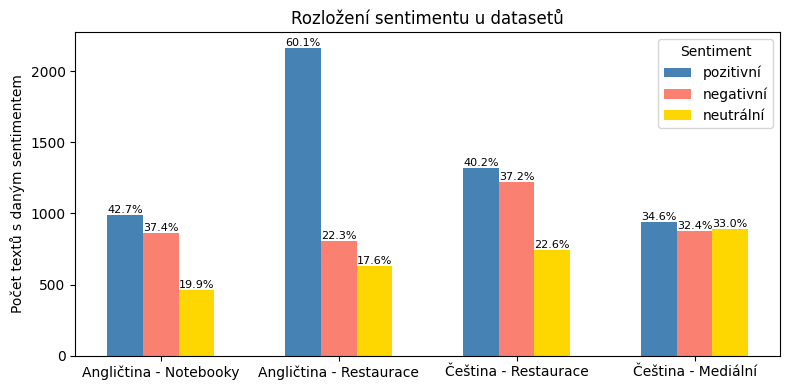
\includegraphics[width=0.9\textwidth]{images/sentiment-distribution}
    \caption[Rozdělení sentimentu v datasetech]%
    {Rozdělení sentimentu v datasetech, vlastní práce}
    \label{fig:SentimentDistribution}
\end{figure}

Pro správné použití datasetů při trénování modelů bylo nejprve nutné každý korpus rozdělit na tři části: \emph{trénovací}, \emph{validační} a \emph{testovací}. Ve všech případech byl zachován jednotný poměr -- 70~\% dat bylo použito pro trénování, 20~\% pro validaci a 10~\% pro závěrečné testování. Předběžné dělení dat zajistí, že všechna následná trénování modelů využijí stejnou strukturu korpusu, a tím umožní objektivně porovnávat dosažené výsledky, protože trénování i vyhodnocení každého modelu proběhne nad totožnými, předem definovanými množinami.

\subsection{Dataset SemEval-2014}
Tato datová sada patřila k prvním, jež se soustředily na aspektovou analýzu sentimentu (ABSA). Do té doby se většina dostupných souborů pro analýzu sentimentu zaměřovala spíše na celkovou náladu či postoj v úrovni celé věty nebo dokumentu. Proto se tým za tímto projektem rozhodl připravit dvě samostatné kolekce recenzí -- jednu zaměřenou na notebooky a druhou na restaurace.~\cite{pontiki-etal-2014-semeval}

Oba datasety byly anotovány dvěma anotátory: jeden byl studentem magisterského studia a druhý odborníkem na lingvistiku. V případě neshod mezi těmito anotátory zasáhl třetí, expertní anotátor. Nejčastější neshody spadaly do jednoho z následujících tří typů: \emph{Nejasnost polarity} (Polarity ambiguity), \emph{Hranice víceslovných aspektů} (Multi-word aspect term boundaries), a \emph{termín aspektu versus odkaz na cílovou entitu} (Aspect term vs. reference to target entity). Podrobnější popis těchto typů a vytváření celého datasetu je uveden v jejich práci~\cite{pontiki-etal-2014-semeval}.

\subsubsection{Recenze notebooků}
Jak již bylo zmíněno, tento dataset byl představen v díle~\cite{pontiki-etal-2014-semeval}. Samotná data však byla získána z portálu Hugging Face, kde je připravil Tom Aarsen a jsou dostupná z~\cite{TomLaptops}.

V datasetu recenzí notebooků je celkem 2313 vzorků, rozdělených na 1619 trénovacích, 462 validačních a 232 testovacích. Tento dataset obsahuje 1456 unikátních textů a 1031 unikátních aspektů. Rozdělení sentimentu v tomto datasetu je znázorněno v grafu~\ref{fig:SentimentDistribution}. Průměrná délka textu činí 104,8 znaků, což odpovídá přibližně 19,3 slovům. Nejdelší text má 464 znaků (nebo 78 slov). Celkové rozložení délky textu je zobrazeno v grafu~\ref{fig:LaptopLenDistribution}.

\begin{figure}[ht]
    \centering
    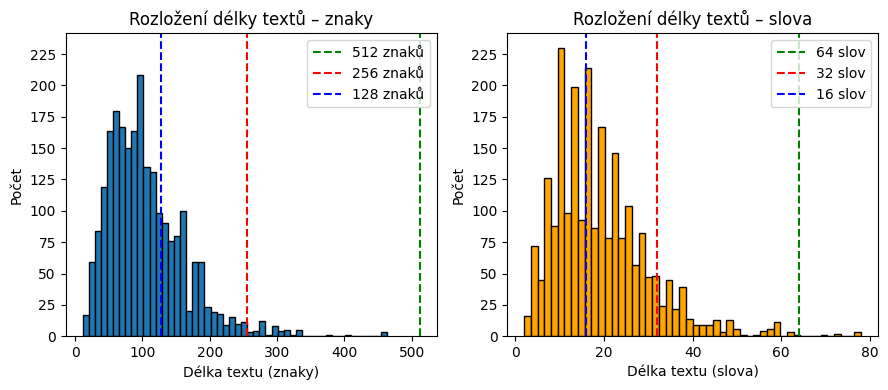
\includegraphics[width=0.9\textwidth]{images/Laptops-distribution}
    \caption[Rozdělení délky textů v datasetu Recenze notebooků v angličtině]%
    {Rozdělení délky textů v datasetu Recenze notebooků v angličtině, vlastní práce}
    \label{fig:LaptopLenDistribution}
\end{figure}

Mezi nejčastější aspekty v tomto datasetu patří: \emph{screen} (obrazovka), \emph{use} (použití) a \emph{price} (cena). Pro tento dataset bylo testováno použití různých tokenizátorů, aby se zjistila ideální délka vstupních sekvencí pro modely. Maximální délky tokenizovaných sekvencí se pohybovaly v rozmezí 97 až 192 tokenů. Tento velký rozptyl je způsoben tím, že na anglický dataset byly použity i tokenizátory, které byly trénovány pouze na češtině, což vedlo k rozdílným výsledkům. Největší rozdíl v délkách tokenizovaných textů je zobrazen v grafu~\ref{fig:LaptopToken}. Podrobné srovnání tokenizátorů bude uvedeno v kapitole~\ref{Results}. Další grafy pro všechny použité tokenizátory a podrobné statistiky tohoto datasetu lze nalézt v souboru \uv{Laptop-English.ipynb}.

\begin{figure}[ht]
    \centering
    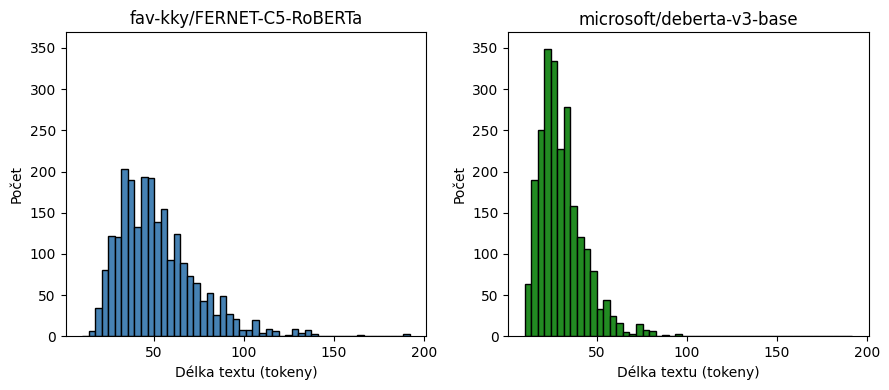
\includegraphics[width=0.9\textwidth]{images/LaptopToken}
    \caption[Porovnání dvou tokenizátorů na datasetu Recenze notebooků v angličtině]%
    {Porovnání dvou tokenizátorů na datasetu Recenze notebooků v angličtině, vlastní práce}
    \label{fig:LaptopToken}
\end{figure}

\subsubsection{Recenze restaurací}
Data pro dataset recenzí restaurací byla také získána z portálu Hugging Face, kde je opět připravil Tom Aarsen, a jsou dostupná z~\cite{TomRestaurants}. Díky tomu, že datasety byly připraveny jedním autorem, je mezi daty zachována konzistence.

Tento dataset obsahuje 3602 vzorků, což ho činí podstatně větším než dataset recenzí notebooků. Vzorky jsou rozděleny na 2521 trénovacích, 720 validačních a 361 testovacích. Tento dataset obsahuje 1976 unikátních textů a 1268 unikátních aspektů. Rozdělení sentimentu v tomto datasetu je zobrazeno v grafu~\ref{fig:SentimentDistribution}. Je zde patrné, že pozitivní data převyšují negativní téměř trojnásobně, což znamená, že modely trénované na těchto datech budou mít tendenci predikovat pozitivní sentiment. Proto se dá předpokládat, že celková přesnost bude výší než u modelů trénovaných na jiných datech. Průměrná délka textu v tomto datasetu je 96,5 znaku, což odpovídá přibližně 17,5 slovům. Nejdelší text má 357 znaků (69 slov). Celkové rozložení délky textu je znázorněno v grafu~\ref{fig:RestaurantLenDistribution}.

\begin{figure}[ht]
    \centering
    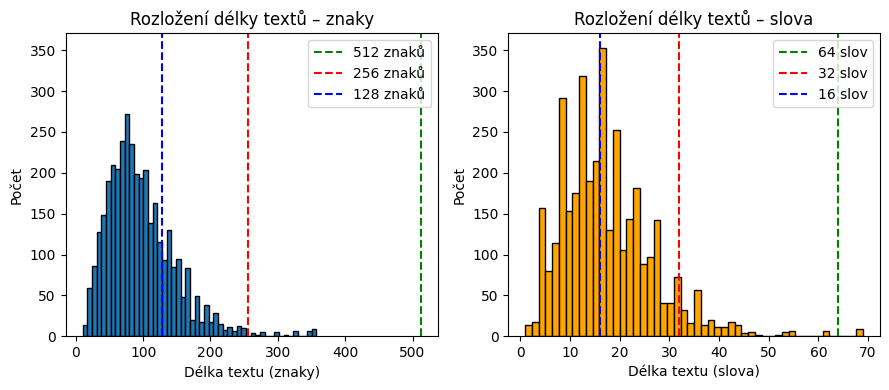
\includegraphics[width=0.9\textwidth]{images/restaurants-distribution}
    \caption[Rozdělení délky textů v datasetu Recenze restaurací v angličtině]%
    {Rozdělení délky textů v datasetu Recenze restaurací v angličtině, vlastní práce}
    \label{fig:RestaurantLenDistribution}
\end{figure}

Mezi nejčastější aspekty v tomto datasetu patří: \emph{food} (jídlo) a \emph{service} (obsluha), které se vyskytují mnohem častěji než ostatní aspekty. Pro zjištění ideální délky vstupů pro model bylo provedeno testování různých tokenizátorů. Maximální délky textů po tokenizaci pro jednotlivé tokenizátory se pohybovaly mezi 90 a 149 tokeny. Zde je opět vcelku velký rozsah maximálních délek, zobrazený v grafu~\ref{fig:RestaurantToken}. Další grafy pro všechny použité tokenizátory a další statistiky týkající se tohoto datasetu jsou k dispozici ve zdrojovém kódu v souboru: \uv{Restaurant-English.ipynb}.

\begin{figure}[ht]
    \centering
    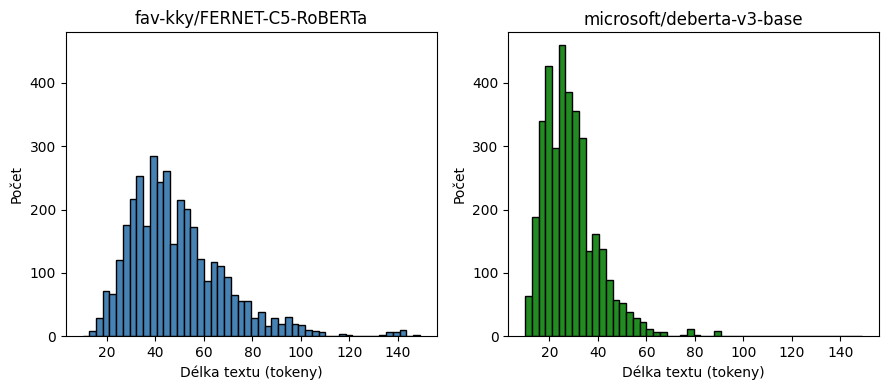
\includegraphics[width=0.9\textwidth]{images/restaurantsToken}
    \caption[Porovnání dvou tokenizátorů na datasetu Recenze restaurací v angličtině]%
    {Porovnání dvou tokenizátorů na datasetu Recenze restaurací v angličtině, vlastní práce}
    \label{fig:RestaurantToken}
\end{figure}

\subsection{Český dataset recenzí restaurací}

Tento dataset vznikl jako česká obdoba datasetu SemEval-2014. Autoři využili recenze restaurací z portálu \url{www.nejezto.cz}, kde vybrali deset podniků s nejvyšším počtem hodnocení. Anotaci provedli tři rodilí mluvčí; podrobnosti o postupu a pravidlech značení jsou popsány v práci~\cite{steinberger-etal-2014-aspect}. Samotná data jsou dostupná v repozitáři~\cite{CzechRestaurants}.

Dataset obsahuje 3281 záznamů, rozdělených na 2296 trénovací, 656 validační a 329 testovací. Z těchto záznamů je 1658 unikátních textů a 1150 unikátních aspektů. Rozdělení polarit sentimentu je zachyceno v grafu~\ref{fig:SentimentDistribution}. Průměrná délka textu činí 124 znaků (přibližně 20,4 slova), nejdelší recenze má 623 znaků (111 slov). Distribuci délek recenzí ukazuje graf~\ref{fig:CzechRestaurantLenDistribution}.

\begin{figure}[ht]
    \centering
    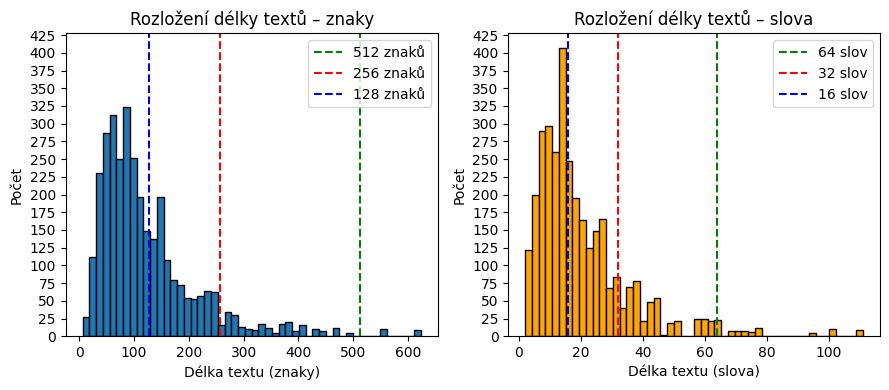
\includegraphics[width=0.9\textwidth]{images/Czechrestaurants-distribution}
    \caption[Rozdělení délky textů v datasetu Recenze restaurací v češtině]%
    {Rozdělení délky textů v datasetu Recenze restaurací v češtině, vlastní práce}
    \label{fig:CzechRestaurantLenDistribution}
\end{figure}

Nejčastěji se v anotacích vyskytují aspekty \emph{jídlo}, \emph{obsluha} a \emph{restaurace}. Mezi deset nejfrekventovanějších patří také tvary \emph{restauraci}, \emph{jídla} či \emph{Jídlo}. Různé pádové tvary ilustrují jednu z komplikací českého jazyka oproti angličtině. Do budoucna by bylo vhodné dataset normalizovat, případně při trénování využít lemmatizaci nebo stemming popsané v sekci~\ref{NLU}.

V tomto datasetu je patrný mnohem větší rozdíl mezi tokenizátory, než v předchozích případech. Maximální délky tokenizovaných sekvencí se pohybovaly v rozmezí od 176 do 358 tokenů. Tento výrazný rozdíl je způsoben tím, že čeština má více znaků, se kterými mají anglické tokenizátory problém. Anglické tokenizátory jsou trénovány primárně na anglických textech a proto mají problém s češtinou, která obsahuje více diakritických znamének a složitější morfologii (např. více pádů). V grafu~\ref{fig:CzechRestaurantToken} je zobrazen největší rozdíl mezi dvěma tokenizátory, který ukazuje tento problém. Grafy pro všechny použité tokenizátory a další statistiky tohoto datasetu jsou k dispozici ve zdrojovém kódu v souboru \uv{Restaurant-Czech.ipynb}.

\begin{figure}[ht]
    \centering
    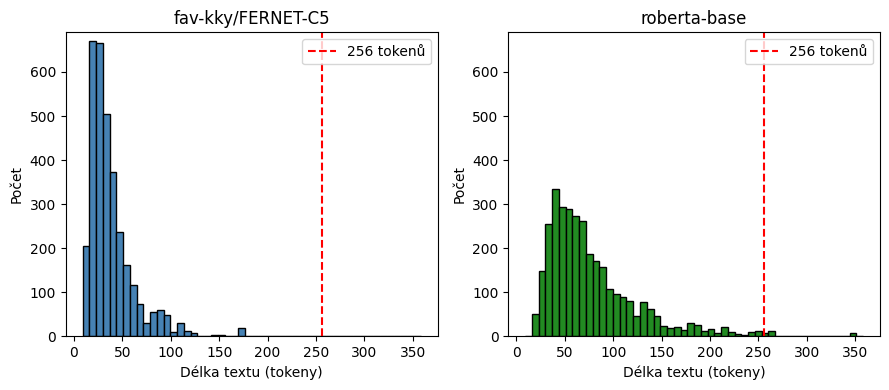
\includegraphics[width=0.9\textwidth]{images/CzechrestaurantsToken}
    \caption[Porovnání dvou tokenizátorů na datasetu Recenze restaurací v češtině]%
    {Porovnání dvou tokenizátorů na datasetu Recenze restaurací v češtině, vlastní práce}
    \label{fig:CzechRestaurantToken}
\end{figure}

\subsection{Data z mediální domény}\label{datasetmedia}
Původně měla být použita reálná data z archivu Newton Media. Analýza však ukázala, že dostupné korpusy jsou pro trénování jazykových modelů nevhodné -- anotace aspektů jsou nevyvážené a počet tříd výrazně kolísá. Proto byl vytvořen \emph{syntetický} dataset, který byl následně použit pro trénování modelů.

\subsubsection{Popis generování dat}
Data byla vygenerována pomocí modelu Gemini 2.0 Flash~\cite{Gemini}. Proces generování probíhal tak, že z reálných článků byly nejprve vybrány tři nejdůležitější aspekty. Každému z těchto aspektů byl následně přiřazen náhodný sentiment. Poté bylo vytvořeno shrnutí daného článku, přičemž byl kladen důraz na zachování přiřazeného sentimentu k daným aspektům. K extrakci aspektů byl použit prompt uvedený v~\ref{code:prompt}. Pro generování shrnutí s konkrétním sentimentem k těmto aspektům byl následně použit druhý prompt, uvedený v~\ref{code:prompt2}. Přesné použití těchto promptů a celý proces generování lze nalézt v příloze v souboru \uv{script.py}.

\begin{listing}[ht]
\begin{minted}{python3}
f"""Najdi {n} nejdůležitějších, vzájemně odlišných aspektů, 
které se týkají hlavního tématu následujícího textu. Aspekt je 
jednoduché podstatné jméno nebo fráze, která popisuje konkrétní 
vlastnost nebo aspekt daného tématu. Například: „kvalita 
produktu“, „cena“, „zákaznický servis“.
Napiš seznam aspektů, které jsou relevantní pro daný text. 
Nepoužívej žádné úvodní fráze ani vysvětlení, pouze seznam 
aspektů.""""
\end{minted}
\caption[Ukázka promptu pro extrakci nejdůležitějších aspektů]%
{Ukázka promptu pro extrakci nejdůležitějších aspektů, vlastní práce}
\label{code:prompt}
\end{listing}

\begin{listing}[ht]
\begin{minted}{python3}
f"""Následující text se týká několika aspektů: {aspects_repr}.
Napiš souvislé shrnutí (max 200 slov), kde každý aspekt je 
zmíněn a popsán tónem, který mu byl přiřazen (pozitivní/
negativní/neutrální). Snaž se o obecné shrnutí, kde jsou 
aspekty mimochodem zmíněny.
Nezapomeň na žádný aspekt a dbej, aby výsledný odstavec působil 
přirozeně. Pamatuj, že to má být shrnutí, ne analýza! I kdyby 
byl aspekt v textu zmíněň například s jiným tónem než zadáno, 
shrnutí by mělo být v souladu s tónem zadaným v úkolu a nikoli 
s tónem v textu.""""
\end{minted}
\caption[Ukázka promptu pro generaci shrnutí]%
{Ukázka promptu pro generaci shrnutí, kde se dbá na daný sentiment k daným aspektům, vlastní práce}
\label{code:prompt2}
\end{listing}

\subsubsection{Popis samotného datasetu}
Po finálních úpravách obsahuje dataset 2709 záznamů, rozdělených na 1896 trénovacích, 542 validačních a 271 testovacích instancí. Celkem zahrnuje 903 unikátních textů a 1681 aspektů. Polaritní rozložení je vyvážené (graf~\ref{fig:SentimentDistribution}), což eliminuje zkreslení při trénování modelů. Průměrná délka textu činí 529,2 znaku, přibližně 75,5 slova, nejdelší text dosahuje 862 znaků (125 slov). Distribuci délek ukazuje graf~\ref{fig:CzechMediaLenDistribution}. Oproti předchozím datasetům jsou texty podstatně delší, což odpovídá charakteru mediálních článků.

\begin{figure}[ht]
    \centering
    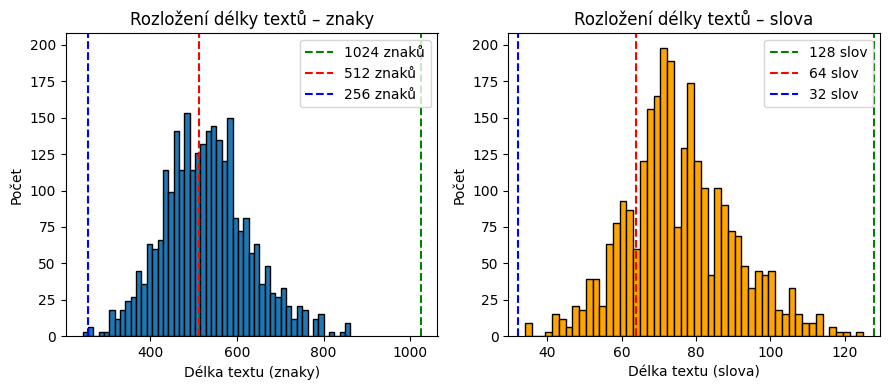
\includegraphics[width=0.9\textwidth]{images/Czechmedia-distribution}
    \caption[Rozdělení délky textů v datasetu Mediální texty v češtině]%
    {Rozdělení délky textů v datasetu Mediální texty v češtině, vlastní práce}
    \label{fig:CzechMediaLenDistribution}
\end{figure}

Nejfrekventovanějšími aspekty v celém korpusu jsou \emph{coming out}, \emph{dlouholetý vztah} a \emph{příčina výpadku}; žádný z nich však nevyčnívá svou absolutní četností natolik, aby převážil nad ostatními. V tomto datasetu je rozdíl mezi tokenizátory ještě výraznější než u dříve popsaných sad -- maximální délky tokenizovaných sekvencí se pohybovaly od 170 do 482 tokenů. Graf~\ref{fig:CzechMediaToken} ukazuje kontrast mezi dvojicí tokenizátorů stejné architektury RoBERTa~\cite{liu2019robertarobustlyoptimizedbert}: česká varianta dosahuje svých nejdelších sekvencí přibližně na úrovni nejkratších sekvencí anglické verze, což dokládá, že anglické tokenizátory si s češtinou poradí podstatně hůře. Další grafy délek po tokenizaci a doplňkové statistiky k tomuto korpusu jsou k dispozici v přiloženém notebooku \uv{Media‑Czech.ipynb}.

\begin{figure}[ht]
    \centering
    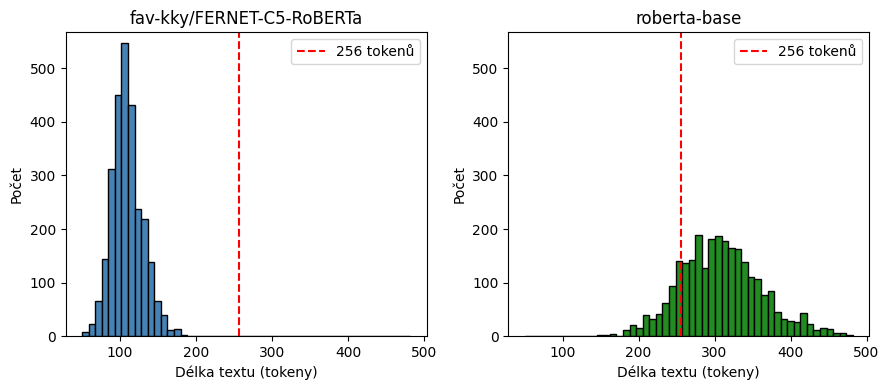
\includegraphics[width=0.9\textwidth]{images/CzechmediaToken}
    \caption[Porovnání dvou tokenizátorů na datasetu Mediální texty v češtině]%
    {Porovnání dvou tokenizátorů na datasetu Mediální texty v češtině, vlastní práce}
    \label{fig:CzechMediaToken}
\end{figure}

\section{Vybrané metody}\label{VybMet}
Využití BERT modelů pro ABSA se zabývali autoři článku~\cite{sun-etal-2019-utilizing}, kteří představili čtyři nová řešení zaměřená specificky na TASD a E2E-ABSA. Využívají vlastnost modelu BERT, konkrétně jeho struktura vstupu, díky čemuž je možné převést úkoly ABSA (ať už jakékoliv podúlohy) na klasifikaci dvojice vět (\emph{sentence-pair classification}). Tento přístup bude testován i v této práci, kde bude porovnávána klasifikace dvojice vět s klasifikací jedné věty (\emph{single-sentence classification}).

Při převodu ABSA úloh na klasifikaci dvojice vět se druhá věta používá jako doplňující informace k získání sentimentu z původního textu. Jedna věta je původní text a druhá slouží jako doplňující (\emph{auxiliary sentence}). Tato pomocná věta může být formulována buď jako otázka (\emph{QA}), nebo jako pseudo-věta (\emph{NLI}). Tyto dva přístupy se pak dále dělí podle toho, zda bude odpovědí polarita sentimentu (\emph{M}), nebo odpověď typu ano/ne (\emph{B})~\cite{sun-etal-2019-utilizing}.
\begin{itemize}
    \item \textbf{QA-M} \\
    Doplňující věta je ve formě otázky, na kterou bude odpověď už daná polarita sentimentu. Příklad otázky: \uv{Jaký je sentiment tohoto aspektu: \{aspect\}?}, kde za \{aspect\} může být dosazen libovolný požadovaný aspekt z daného textu.
    \item \textbf{NLI-M} \\
    Doplňující věta v tomto případě nemá přísná pravidla a jedná se o tzv. pseudo-větu. Může jít například o větu jako: \uv{aspekt: \{aspect\}}. Model pak vrací polaritu sentimentu na základě této věty.
    \item \textbf{QA-B} \\
    Doplňující věta je opět ve formě otázky, ale úloha je převedena na binární odpověď (ano/ne). Polarita sentimentu může mít tři možné hodnoty: \uv{pozitivní}, \uv{negativní} a \uv{neutrální}. V této metodě je třeba vygenerovat tři různé otázky pro jeden text, což znamená, že predikce musí být provedena třikrát, aby byly získány odpovědi pro všechny tři polarity. Příklad možných otázek: \uv{Je sentiment pro aspekt: \{aspect\} pozitivní?}, \uv{Je sentiment pro aspekt: \{aspect\} negativní?} a \uv{Je sentiment pro aspekt: \{aspect\} neutrální?}.
    \item \textbf{NLI-B} \\
    Opět jde o pseudo-větu, která však již obsahuje informaci o sentimentu. Opět bude potřeba vygenerovat tři věty pro jeden text. Příklad takových vět: \uv{aspekt: \{aspect\}, sentiment: pozitivní}, \uv{aspekt: \{aspect\}, sentiment: negativní}, \uv{aspekt: \{aspect\}, sentiment: neutrální}.~\cite{sun-etal-2019-utilizing}
\end{itemize}

Jak již bylo zmíněno, v této práci budou použity dvě metody: jedna pro klasifikaci jedné věty a druhá pro klasifikaci dvojice vět. Pro klasifikaci dvojice vět bude z metod popsaných výše vybrána metoda \emph{QA-M}. Tato metoda byla zvolena na základě pozorování v práci~\cite{sun-etal-2019-utilizing}, která ukázala, že metody typu \emph{QA} dosahovaly lepších výsledků při predikci sentimentu. Verze \emph{M} byla vybrána kvůli její jednoduchosti a menší náročnosti na trénování (u verze \emph{B} by trénování trvalo třikrát déle). Popis implementace těchto metod bude uveden v sekci~\ref{PristupToken}.

\section{Vybrané modely}\label{Modely}
Tato část představuje všechny modely testované v rámci této práce a vysvětluje jejich rozdělení do dvou logických skupin. Mezi nimi bude vybírán nejvhodnější kandidát pro český mediální prostor a na každý z nich se aplikují obě metody popsané v sekci~\ref{VybMet}. Všechny modely jsou založeny na transformátorové architektuře a vycházejí z modelu BERT, který je rovněž součástí této práce.

Modely jsou rozděleny na \emph{inovativní} a \emph{jazykově adaptované}. První skupinu tvoří architektury, které přinášejí nové předtrénovací postupy či mechanismy (např.\ RoBERTa, DeBERTa-V3, ModernBERT). Do druhé skupiny patří verze již existujících modelů přetrénované pro konkrétní jazyková prostředí, zejména pro češtinu a další slovanské jazyky (SlavicBERT, Czert, RobeCzech, FERNET).

Pro popis těchto modelů jsou používány následující parametry: \emph{počet vrstev L} (počet transformátorových bloků), \emph{velikost skrytého vektoru H} (velikost vektoru, který reprezentuje jednotlivé tokeny v každé vrstvě transformátoru) a \emph{počet self-attention hlav A} (počet nezávislých mechanismů pozornosti, které model používá k výpočtu pozornosti pro každý token vzhledem k ostatním tokenům)~\cite{devlin2019bert}. Vypsané parametry všech modelů lze nalézt v tabulce~\ref{tab:modely}.

\begin{table}[ht]
    \centering
    \begin{tabular}{|l|c|c|c|c|}
        \hline
        \textbf{model} & \textbf{L} & \textbf{H} & \textbf{A} & \textbf{počet parametrů}  \\ \hline
        bert-base-uncased & 12 & 768 & 12 & 110 milionů \\ \hline
        bert-large-uncased & 24 & 1024 & 16 & 340 milionů \\ \hline
        bert-base-multilingual-cased & 12 & 768 & 12 & 110 milionů \\ \hline
        roberta-base & 12 & 768 & 12 & 125 milionů \\ \hline
        xlm-roberta-base & 12 & 768 & 12 & 270 milionů \\ \hline
        xlm-roberta-large & 24 & 1024 & 16 & 550 milionů \\ \hline
        deberta-v3-base & 12 & 768 & 12 & 184 milionů \\ \hline
        ModernBERT-base & 22 & 768 & 12 & 149 milionů \\ \hline
        ModernBERT-large & 28 & 1024 & 16 & 395 milionů \\ \hline\hline
        bert-base-bg-cs-pl-ru-cased & 12 & 768 & 12 & 180 milionů \\ \hline 
        Czert-B-base-cased & 12 & 768 & 12 & 110 milionů \\ \hline
        robeczech-base & 12 & 768 & 12 & 126 milionů \\ \hline
        FERNET-C5 & 12 & 768 & 12 & 164 milionů \\ \hline
        FERNET-C5-RoBERTa & 12 & 768 & 12 & 124 milionů \\
        \hline
    \end{tabular}
    \caption{Parametry použitých modelů}
    \label{tab:modely}
\end{table}

\subsection{Inovativní modely}
Následující podsekce popisují modely, které posouvají možnosti transformátorových architektur prostřednictvím nových trénovacích technik, modifikované pozornosti či efektivnější implementace. Tyto inovace mají za cíl zvýšit přesnost, zrychlit rozhodování a snížit paměťové nároky, což je klíčové zejména při zpracování rozsáhlých textových korpusů.

\subsubsection{BERT}
Model BERT (zkratka pro \emph{Bidirectional Encoder Representations from Transformers}) byl představen v práci~\cite{devlin2019bert} jako řešení pro široké spektrum úloh na úrovni věty a tokenu (sentence-level and token-level tasks). Předchozí modely byly zaměřeny pouze na jeden směr čtení textu, zatímco BERT, díky své \emph{dvojcestné} (bidirectional) architektuře, dokáže zohlednit kontext z obou stran textu, což zlepšuje predikci tokenů. BERT je předtrénovaný model, který se nejprve trénuje na obecných datech a poté je možné jej doladit (fine-tune) na specifických úlohách s menšími datovými sadami.

BERT je postaven na transformátorové architektuře, která byla představena v sekci~\ref{Transformator}, využívající model encoder, popsán v sekci~\ref{DECENC}. Vstupy do modelu BERT mohou být jak jednotlivé věty, tak dvojice vět (například otázka a odpověď). Tato flexibilita rozšiřuje možnosti využití modelu, jak je tomu i v této práci. Pro předtrénování modelu BERT byly použity dva rozsáhlé datasety: BooksCorpus (800 milionů slov) a anglická Wikipedie (2,5 miliardy slov). Předtrénovací techniky zahrnovaly \emph{Missing token prediction} a \emph{Next sentence prediction}, které jsou podrobněji popsány v sekci~\ref{predtrenovani}. Podrobnější popis modelu BERT lze nalézt v díle~\cite{devlin2019bert}.

V této práci byly použity dvě verze modelu BERT: \emph{bert-base-uncased}~\cite{BERTbaseuncased} a \emph{bert-large-uncased}~\cite{BERTlargeuncased}. Jedná se o stejné modely, lišící se pouze velikostí. Větší modely jsou schopny zachytit složitější vlastnosti textu, ale jsou výpočetně náročnější.~\cite{devlin2019bert} Zvoleny byly \emph{uncased} verze, protože patří k nejpoužívanějším anglickým modelům BERT a v praxi se nasazují častěji než jejich \emph{cased} protějšky (\emph{bert-base-cased}~\cite{BERTbasecased} a \emph{bert-large-cased}~\cite{BERTlargecased}).

\subsubsection{mBERT}
Model \emph{multilingual BERT} (mBERT) vychází ze stejné architektury jako původní anglický BERT; liší se pouze trénovacími daty. Byl trénován na Wikipediích ve 100 jazycích s největším počtem článků. Rozložení dat mezi jazyky je však nerovnoměrné -- například angličtina tvoří přibližně 21~\% veškerých trénovacích dat. Aby i jazyky s omezenými zdroji (\emph{low-resource} jazyky) získaly dostatečné zastoupení, autoři použili vyvážené vzorkové (sample) schéma. Podrobné informace jsou uvedeny v repozitáři projektu~\cite{GoogleResearchGitHubMulti}.

mBERT nemá \emph{large} variantu, proto je v této práci použit model \emph{bert-base-multilingual-cased}~\cite{mBERTbasecased}. Verze \emph{cased} je doporučena tvůrci modelu, protože opravuje normalizační problémy u mnoha jazyků, speciálně je doporučena pro jazyky, které nepoužívají latinku (většinou je lepší i pro jazyky, které latinku používají).~\cite{GoogleResearchGitHubMulti}

\subsubsection{RoBERTa}
Model RoBERTa (\emph{Robustly Optimized BERT Pretraining Approach}) vznikl na základě zjištění, že původní BERT je ve fázi předtrénování nedostatečně využit. Autoři proto navrhli několik úprav předtrénovacího postupu:

\begin{enumerate}
    \item delší trénování na rozsáhlejších datech,
    \item odstranění \emph{Next Sentence Prediction},
    \item trénování na delších sekvencích,
    \item dynamickou změnu maskovacího vzoru v průběhu trénování.
\end{enumerate}

Díky uvedeným úpravám dosahuje RoBERTa ve srovnání s původním modelem BERT-em výrazně lepších výsledků napříč různými jazykovými úlohami. Podrobné zdůvodnění jednotlivých vylepšení a jejich vliv na výkon modelu je rozebráno v původním článku~\cite{liu2019robertarobustlyoptimizedbert}.

V této práci je použit model \emph{roberta-base}~\cite{RoBERTabase}. RoBERTa se nečlení na varianty \emph{cased} a \emph{uncased}, takže nebylo nutné volit mezi různými verzemi.

\subsubsection{XLM-RoBERTa}
XLM-RoBERTa je vícejazyčný model navržený jako nástupce mBERT pro vícejazyčné úlohy. Vznikl kombinací optimalizovaného předtrénovacího postupu z modelu RoBERTa a techniky předtrénování XLM (\emph{cross-lingual language models}, vícejazyčné jazykové modelování) představené v práci~\cite{lample2019crosslinguallanguagemodelpretraining}. Výsledkem je model schopný pracovat se 100 jazyky, který překonává předešlé nejlepší modely. Podrobnosti o architektuře a trénování jsou popsány v~\cite{conneau2020unsupervisedcrosslingualrepresentationlearning}.

V této práci jsou použity obě dostupné velikosti: \emph{xlm-roberta-base}~\cite{XLMRoBERTabase} a \emph{xlm-roberta-large}~\cite{XLMRoBERTalarge}. Jde o jediný vícejazyčný model v této práci, který je k dispozici i ve variantě \emph{large}.

\subsubsection{DeBERTa-V3}
Modelová architektura DeBERTa (\emph{Decoding-enhanced BERT with disentangled attention}) rozšiřuje možnosti BERT a RoBERTa dvěma hlavními inovacemi. První z nich je rozdělená pozornost (\emph{disentangled attention}): každé slovo je reprezentováno dvojicí vektorů -- jeden nese obsahovou informaci, druhý relativní pozici -- a váhy pozornosti se počítají odděleně pro obsahové a polohové složky. Druhou novinkou je vylepšený maskovací dekodér, jenž do předtrénování začleňuje i absolutní pozice tokenů. Podrobnosti těchto inovací uvádí práce~\cite{he2021debertadecodingenhancedbertdisentangled}.

Tato práce využívá novější variantu \emph{DeBERTa-V3}, jež nahrazuje klasickou techniku předtrénování predikce chybějícího tokenu (\emph{missing token prediction}) technikou predikce vyměněného tokenu (\emph{replaced token detection}). Také je zde představena nová metoda \emph{gradient-disentangled embedding sharing}, která zlepšuje efektivnost trénování a celkovou kvalitu modelu. Při stejném předtrénovacím režimu jako původní DeBERTa tato vylepšení ukazují zlepšení na širokém spektru NLU úloh. Podrobnější popis těchto vylepšení lze nalézt v díle~\cite{he2023debertav3improvingdebertausing}.

Použitým modelem je \emph{deberta-v3-base}~\cite{DeBERTav3base}. Existuje i vícejazyčná varianta mDeBERTa-V3, ta však pokrývá pouze 16 jazyků a čeština mezi nimi chybí, proto není v této práci použita.

\subsubsection{ModernBERT}
ModernBERT představuje nejnovější encoder-only model vycházející z původního BERT-u. Autoři do klasické transformátorové architektury postupně začlenili řadu ověřených novinek a přidali vlastní úpravy zaměřené na efektivitu jak z hlediska rychlosti, tak paměťové náročnosti. Současně optimalizovali implementaci pro trénování na GPU. Podrobný popis všech změn je uveden v práci~\cite{warner2024smarterbetterfasterlonger}.

Ve srovnání s dřívějšími modely (např. DeBERTa) je ModernBERT výrazně úspornější a typicky alespoň dvakrát rychlejší; v některých úlohách autoři uvádějí až čtyřnásobné zrychlení při současném snížení paměťových nároků. Další zásadní předností je maximální kontextová délka 8192 tokenů, tedy téměř šestnáctinásobek běžného limitu 512 tokenů. Přehled měřených vlastností a praktická srovnání shrnuje blogový článek~\cite{modernbertreplacment}.

V této práci jsou otestovány obě velikosti modelu, \emph{ModernBERT-base}~\cite{ModernBERTbase} a \emph{ModernBERT-large}~\cite{ModernBERTlarge}. Vícejazyčná varianta zatím neexistuje; kdyby byla k dispozici, nabízela by ideální kombinaci dlouhého kontextu a mnohojazyčné podpory pro analýzu rozsáhlých mediálních textů.

\subsection{Jazykově adaptované modely}
Tato podsekce se věnuje variantám, které nepřinášejí nové architektonické prvky, ale rozšiřují stávající modely na méně zastoupené jazyky -- zde především na češtinu a další slovanské jazyky. Jejich hlavním přínosem je tedy jazyková adaptace, využívají osvědčené inovace z předchozí skupiny a převádějí je do jazykového prostředí, kde původní anglické a vícejazykové modely nedosahují optimální výkonnosti.

\subsubsection{SlavicBERT}
SlavicBERT patří mezi první specializované varianty BERT-u zaměřené na slovanské jazyky (češtinu, ruštinu, polštinu a bulharštinu). Autoři vyšli z modelu \emph{mBERT} a dále jej doladili na korpusech výhradně v těchto čtyřech jazycích, protože trénovat novou architekturu od začátku by bylo výpočetně i finančně nákladné. Původně byl model navržen pro rozpoznávání vícejazyčných pojmenovaných entit (NER, named entity recognition), nicméně je použitelný i pro další úlohy zpracování přirozeného jazyka~\cite{arkhipov-etal-2019-tuning}.

V této práci je využita verze \emph{bert-base-bg-cs-pl-ru-cased}~\cite{SlavicBERThug}, která je na portálu Hugging Face dostupná jako jediná oficiálně zveřejněná varianta.

\subsubsection{Český BERT -- Czert}\label{Czert}
Cílem autorů modelu Czert bylo vytvořit model vycvičený výhradně na českých datech. Na rozdíl od SlavicBERT-u zvolili trénování \emph{od nuly}, aby se model učil jazyk čistě z českého korpusu. K předtrénování použili přibližně 36 GB textu. Architektura i postup kopírují původní BERT, jedinou úpravu vyžadovala technika \emph{Next Sentence Prediction}: vzhledem ke krátkým textovým blokům často chyběla vhodná následující věta, což autoři řešili v detailech popsaných v práci~\cite{sido2021czertczechbertlike}.

Vznikly dvě varianty: \emph{Czert-B} založená na BERT-u a lehčí \emph{Czert-A} vycházející z ALBERT-u. Pro tuto práci je zvolen model \emph{Czert-B-base-cased}~\cite{CzertHugging}, jehož rozměry odpovídají mBERT-u a usnadňují tak férové porovnání s ostatními modely.

\subsubsection{Český RoBERTa -- RobeCzech}\label{RobeCzech}
Na dosavadní český model založený na architektuře BERT (Czert) navázal model RobeCzech, jenž vychází z architektury RoBERTa. Předtrénování proběhlo na souboru českých korpusů o celkovém rozsahu převyšujícím čtyři miliardy tokenů a k tréninku byl použit oficiální kódový rámec pro RoBERTa. Následně byl RobeCzech doladěn a vyhodnocen na pěti úlohách z oblasti NLP, mezi nimiž byla i klasická (ne-aspektová) analýza sentimentu. Ve všech sledovaných úlohách překonal ostatní modely stejné velikostní kategorie. Podrobný popis korpusu, parametrů trénování i výsledků benchmarku je uveden v práci~\cite{Straka_2021}.

V této práci se používá \emph{robeczech-base}~\cite{RobeCzech}; jedná se o jedinou dosud publikovanou varianta tohoto modelu, další verze zatím nebyly vytvořeny.

\subsubsection{Český BERT a RoBERTa -- FERNET}\label{FERNET}
Název FERNET zastřešuje dvojici českých modelů, jejichž cílem bylo rozšířit portfolio dostupných jazykových modelů pro češtinu. Autoři zvolili jiné předtrénovací korpusy než u předchozích modelů Czert a RobeCzech -- konkrétně vlastní korpusy \emph{Czech News} a \emph{C5}, jenž představuje českou obdobu anglického C4~\cite{JMLR:v21:20-074}. Na těchto datech vznikly dvě varianty: \emph{FERNET-C5}, vycházející z architektury BERT, a \emph{FERNET-News}, založená na architektuře RoBERTa. Oba modely byly po jemném doladěním srovnány na dvou úlohách z oblasti NLP, z nichž jedna byla opět klasická analýza sentimentu; v tomto srovnání dosáhl FERNET-C5 nejlepších výsledků mezi dostupnými českými modely. Detailní popis přípravy dat, parametrů trénování a dosažených skóre přináší studie~\cite{Lehe_ka_2021}.

V této práci budou využity dvě varienty: \emph{FERNET-C5}~\cite{FERNET-C5} a \emph{FERNET-C5-RoBERTa}~\cite{FERNET-C5-RoBERTa}. Druhý model, ačkoli nebyl součástí původního článku, je model založený na architektuře RoBERTa, který byl předtrénován jak na datasetu C5, tak na datasetu českých novinek.

\section{Popis přístupu}
V předchozích částech byly podrobně představeny použité datasety, metody i jazykové modely. Tato sekce vysvětluje, \emph{jak} byly všechny tyto komponenty propojeny v praxi. Popisuje trénovací prostředí, klíčové knihovny a důležité fragmenty kódu, které zajišťují trénování a vyhodnocení modelů.

\subsection{Trénovací prostředí}
Veškeré trénování probíhalo v prostředí Google Colab \cite{GoogleColab} -- hostovaném Jupyter notebooku -- který poskytuje zdarma přístup k výpočetním zdrojům, včetně GPU a TPU. Tato varianta je pro akademické účely výhodná, protože odstraňuje nutnost vlastnit výkonný hardware.

V Colabu (ve verzi použité během trénování) byl využit virtuální stroj s~12{,}7 GB systémové RAM a grafickou kartou \emph{NVIDIA Tesla T4} \cite{T4Nvidia} s 15 GB paměti. Přestože T4 není nejvýkonnější čip v nabídce Colabu, poskytla dostatečný výkon. Všechny modely bylo možné natrénovat bez placeného tarifu a bez nutnosti zkracovat dávky či redukovat maximální délku vstupu.

\subsection{Použité knihovny}
Tato podsekce stručně charakterizuje knihovny využité při implementaci trénování. Všechny moduly jsou součástí ekosystému \emph{Hugging Face}~\cite{huggingface} nebo patří mezi standardní nástroje pro práci s daty a hluboké učení.

\begin{itemize}
    \item \textbf{Datasets}~\cite{HuggDatasets}\\
    Knihovna \emph{Datasets} usnadňuje stahování, ukládání a transformaci datových sad. V rámci práce je používána datová struktura \emph{Dataset}, do níž jsou načteny trénovací, validační a testovací podmnožiny.

    \item \textbf{pandas}~\cite{pandas} a \textbf{NumPy}~\cite{numpy}\\
    Základní nástroje pro manipulaci s tabulkovými daty (\emph{pandas}) a efektivní matematické operace (\emph{NumPy}).

    \item \textbf{Transformers}~\cite{HuggTransformers}\\
    Klíčová knihovna poskytující rozhraní k předtrénovaným modelům, tokenizátorům a trénovacím nástrojům. Umožňuje rychlé jemné doladění (\emph{fine-tuning}) modelů i jejich trénování od začátku.

    \item \textbf{Evaluate}~\cite{HuggEvaluate}\\
    Modul s implementacemi vyhodnocovacích metrik; ve spojení s \emph{Transformers} zajišťuje jednotný rámec pro sledování výkonu při trénování.

    \item \textbf{PyTorch}~\cite{PyTorch}\\
    Framework hlubokého učení použitý jako backend pro trénování a učení neuronových sítí.
\end{itemize}

\subsection{Popis částí kódu}
Tato podsekce se zaměřuje na klíčové fragmenty zdrojového kódu, který byl použit při trénování jednotlivých modelů. Veškeré trénování probíhalo pomocí stejného trénovacího kódu, což zajišťuje konzistenci a reprodukovatelnost výsledků. Dále jsou vysvětleny parametry použité při trénování a upozorněno na odlišnosti mezi oběma aplikovanými metodami. Podsekce rovněž ukazuje funkci, která pro zadaný text a aspekt vrátí odpovídající sentiment. Kompletní skripty pro všechny modely jsou k dispozici v příloze této práce.

\subsubsection{Tokenizace}\label{PristupToken}
Knihovna \emph{Transformers} umožňuje načíst všechny podporované tokenizátory jedním příkazem a okamžitě je použít. Funkce uvedené v kódech~\ref{code:tokenizace} a~\ref{code:tokenizaceQA} zajišťují tokenizaci pro obě zvolené metody; liší se pouze způsobem předání vstupu, ostatní argumenty zůstávají totožné.

\begin{itemize}
    \item \textbf{Základní metoda} (ukázka~\ref{code:tokenizace}): tokenizátor obdrží jediný řetězec složený z \emph{aspect} a \emph{text}.  
    \item \textbf{Metoda QA-M} (ukázka~\ref{code:tokenizaceQA}): první věta obsahuje původní text, druhá věta je dotaz typu \uv{Jaký je sentiment tohoto aspektu: \{aspect\}?} V anglické variantě je otázka přeložena do angličtiny.
\end{itemize}

Jak ukazuje analýza dat v sekci~\ref{datasety}, většina textů se po tokenizaci vejde do 256 tokenů. Výjimkou jsou ale české datasety zpracované tokenizátory netrénovanými na češtině, kde délka tokenizovaných textů byla delší než 256 tokenů. Jenže takové modely nejsou relevantní, neboť nejsou pro češtinu optimalizovány a nejsou od nich očekávané kvalitní výsledky na českých datech. Z tohoto důvodu a k zachování konzistence při trénování různých modelů je maximální délka tokenizovaného textu omezena na \emph{256 tokenů}. 

\begin{listing}[ht]
\centering
\begin{minted}{python3}
def tokenize_function(example):
    combined_input = f"aspect: {example['aspect']} text: \
    {example['text']}"

    encoding = tokenizer(
        combined_input,
        truncation=True,
        padding="max_length",
        max_length=256
    )
    return encoding
\end{minted}
\caption[Ukázka funkce tokenizace u základní metody]%
{Ukázka funkce tokenizace u základní metody, vlastní práce}
\label{code:tokenizace}
\end{listing}

\begin{listing}[ht]
\centering
\begin{minted}{python3}
def tokenize_function(example):
    question_string = f"What is the sentiment of aspect: \
    {example['aspect']}?"

    encoding = tokenizer(
        text=example["text"],
        text_pair=question_string,
        truncation=True,
        padding="max_length",
        max_length=256
    )
    return encoding
\end{minted}
\caption[Ukázka funkce tokenizace u metody QA-M]%
{Ukázka funkce tokenizace u metody QA-M, vlastní práce}
\label{code:tokenizaceQA}
\end{listing}

\subsubsection{Vyhodnocovací metrika}
Jako vyhodnocovací metrika během trénování a pro výběr nejlepší epochy bude použita \emph{přesnost} (accuracy). S využitím knihovny \emph{Evaluate} bude přesnost vypočítána pomocí funkcí uvedenou v ukázce kódu~\ref{code:accuracy}, která je následně předána objektu \emph{Trainer} použitému pro samotné trénování.

\begin{listing}[ht]
\centering
\begin{minted}{python3}
metric = evaluate.load("accuracy")
def compute_metrics(eval_pred):
    logits, labels = eval_pred
    predictions = np.argmax(logits, axis=-1)
    return metric.compute(predictions=predictions, 
                          references=labels)
\end{minted}
\caption[Ukázka funkce pro výpočet přesnosti]%
{Ukázka funkce pro výpočet přesnosti, vlastní práce}
\label{code:accuracy}
\end{listing}

\subsubsection{Trénovací struktura}
Proces trénování je řízen řadou parametrů, které ovlivňují jeho průběh. Aby byla mezi modely zachována srovnatelnost, jsou v celé práci používány totožné hodnoty argumentů; výkonnější hardware by umožnil ladění více kombinací a podrobnější analýzu jejich vlivu na výsledky.

Níže jsou popsány klíčové hyperparametry objektu \emph{TrainingArguments}. Úplný seznam všech podporovaných parametrů je uveden v oficiální dokumentaci~\cite{HuggTrainArg}. Ukázka kódu~\ref{code:trainingarguments} prezentuje konkrétní konfiguraci použitou při trénování všech modelů použitých v této práci.

\begin{itemize}
    \item \textbf{learning\_rate} -- učící parametr, předávaný do optimalizátoru AdamW;
    \item \textbf{num\_train\_epochs} -- počet trénovacích epoch;
    \item \textbf{weight\_decay} -- regularizační složka omezující přeučení (over-fitting);
    \item \textbf{save\_total\_limit} -- maximální počet uložených checkpointů;
    \item \textbf{warmup\_ratio} -- podíl úvodních kroků, v nichž se \emph{learning rate} lineárně zvyšuje z 0 na cílovou hodnotu.
\end{itemize}

\begin{listing}[ht]
\centering
\begin{minted}{python3}
training_args = TrainingArguments(
    output_dir="./results",
    learning_rate=3e-5,
    per_device_train_batch_size=16,
    per_device_eval_batch_size=16,
    num_train_epochs=10,
    weight_decay=0.01,
    eval_strategy="epoch",
    save_strategy="epoch",
    save_total_limit=3,
    logging_dir="./logs",
    logging_steps=200,
    warmup_ratio=0.06,
    load_best_model_at_end=True,
    metric_for_best_model="accuracy"
)
\end{minted}
\caption[Ukázka struktury TrainingArguments]%
{Ukázka struktury TrainingArguments, vlastní práce}
\label{code:trainingarguments}
\end{listing}

Tyto argumenty jsou předány do objektu \emph{Trainer}, ukázaný v~\ref{code:trainer}, jenž zajišťuje vlastní trénování modelu. V parametru \emph{compute\_metrics} je předána funkce pro výpočet zvolené metriky (přesnosti). Samotné trénování se spustí voláním \mintinline{python3}{trainer.train()}.

\begin{listing}[ht]
\begin{minted}{python3}
trainer = Trainer(
    model=model,
    args=training_args,
    train_dataset=train_dataset,
    eval_dataset=val_dataset,
    compute_metrics=compute_metrics
)
\end{minted}
\caption[Ukázka struktury Trainer]%
{Ukázka struktury Trainer, vlastní práce}
\label{code:trainer}
\end{listing}

\subsubsection{Predikace sentimentu}
Jakmile je model natrénován a připraven k použití, je potřeba vytvořit funkci, která umožní jeho aplikaci na nový text. Pro predikci sentimentu pro jeden text a jeden aspekt bude použita funkce uvedená v~\ref{code:prediction}. V této funkci se nejprve provede tokenizace vstupu pomocí stejného tokenizátoru, jaký byl použit při trénování modelu. Poté je tokenizovaný vstup předán do modelu, který vrátí vektor s výsledky pro každou třídu, přičemž pro predikci sentimentu bude vybrána třída s nejvyšší hodnotou.

Ukázka funkce pro modely s klasickou metodou je uvedena v~\ref{code:prediction}. Pro metodu \emph{QA-M} je však nutné provést tokenizaci podle postupu, ukázaného v~\ref{code:tokenizaceQA}.

\begin{listing}[ht]
\begin{minted}{python3}
def predict_sentiment(model, tokenizer, aspect, text):
    combined_input = f"aspekt: {aspect} text: {text}"

    encoding = tokenizer(
        text=combined_input,
        return_tensors="pt",
        truncation=True,
        padding="max_length",
        max_length=256
    )
    with torch.no_grad():
        outputs = model(**encoding)

    logits = outputs.logits
    print(logits)
    predicted_class_id = logits.argmax(dim=1).item()
    return id2label[predicted_class_id]
\end{minted}
\caption[Ukázka funkce na predikci sentimentu]%
{Ukázka funkce na predikci sentimentu, vlastní práce}
\label{code:prediction}
\end{listing}

\section{Vyhodnocovací metriky a praktické testy}
Předchozí sekce byly zaměřeny na trénování jednotlivých modelů -- od popisu použitých metod, přes výběr modelů a datových sad, až po samotný postup trénování. Jakmile však všechny modely budou natrénovány, je nutné vybrat ten nejvhodnější, který bude schopen nejlépe řešit úlohy ABSA.

K tomuto účelu se v této práci uplatňují dva navzájem se doplňující přístupy. Prvním jsou klasické vyhodnocovací metriky: vedle již zmíněné přesnosti se sleduje také makro-F1 a vážené F1 skóre (weighted F1). Druhým přístupem jsou takzvané \emph{praktické testy}, které prověřují schopnost modelů zobecnit na širší tematické okruhy a pracovat i s doménami, jež se v trénovacích datech nevyskytovaly.

\subsection{Vyhodnocovací metriky}\label{metriky}
Vyhodnocovací metriky slouží jako obecný ukazatel kvality modelu, přičemž jsou počítány na testovací množině, tedy na datech, která nebyla použita během samotného trénování. Na základě těchto metrik lze vybrat nejlepší model ze všech natrénovaných modelů na stejném datasetu, protože bude použit stejný dataset na testování kvality.

V této práci budou použity tři metriky: přesnost, macro F1 a vážená F1. Každá z těchto metrik měří jiný aspekt výkonu modelu, a proto je vhodné vyhodnotit všechny tři pro komplexnější popis jednotlivých modelů.

\begin{itemize}
    \item \textbf{Přesnost (accuracy)} -- podíl správně klasifikovaných vzorků z celkového počtu zpracovaných případů~\cite{HuggTrainAcc};
    \item \textbf{F1 skóre} -- harmonický průměr přesnosti (precision) a výtěžnosti (recall).
    \begin{itemize}
        \item \textbf{Macro F1} -- nevážený průměr F1 skóre u všech tříd (label). Tato metrika nezohledňuje nerovnováhu mezi třídami;
        \item \textbf{Vážená F1} -- vážený průměr F1 skóre u všech tříd (label), který bere v úvahu nerovnováhu mezi třídami~\cite{HuggTrainf1}.
    \end{itemize}
\end{itemize}

\subsection{Praktické testy}\label{praktesty}
Klasické metriky, jako je přesnost či~F1~skóre, shrnují výkon modelu jediným číslem a samy o sobě neodhalí, jak si model poradí s konkrétními situacemi. Proto jsou do této práce zařazeny čtyři sady krátkých textů pocházejících z různých domén. Každý text je připraven v angličtině i češtině, aby bylo možné otestovat modely v obou jazycích. V jedné větě se vždy nachází několik aspektů, což umožňuje ověřit, zda model správně rozezná více aspektů v téže větě a přiřadí každému aspektu odpovídající polaritu.

\subsubsection{Recenze notebooků L}
L-sada obsahuje ukázku z domény, na níž byla část modelů přímo trénována, a slouží tedy jako kontrola, zda si tyto modely udrží výhodu i v ručně vytvořeném příkladu. Zároveň umožňuje porovnat jejich výstup s modely, které tréninková data z této oblasti neviděly, a posoudit tak vliv doménového přizpůsobení.

\begin{itemize}
    \item \textbf{Angličtina} \\
    \uv{The \textbf{power} is good, but the \textbf{display} is blurry and dark. The \textbf{battery} was a real surprise, I don't need to charge it during the day!}
    \begin{itemize}
        \item \textbf{L1}: \emph{power} -- pozitivní,
        \item \textbf{L2}: \emph{display} -- negativní,
        \item \textbf{L3}: \emph{battery} -- pozitivní.
    \end{itemize}
    \item \textbf{Čeština} \\
    \uv{\textbf{Výkon} je dobrý, ale \textbf{displej} je rozmazaný a tmavý. \textbf{Baterie} byla skutečným překvapením, nemusím ji přes den nabíjet!}
    \begin{itemize}
        \item \textbf{L1}: \emph{výkon} -- pozitivní,
        \item \textbf{L2}: \emph{displej} -- negativní,
        \item \textbf{L3}: \emph{baterie} -- pozitivní.
    \end{itemize}
\end{itemize}

\subsubsection{Recenze restaurací R}
Stejně jako L-sada pokrývala jednu z trénovacích domén, R-sada se zaměřuje na recenze restaurací, druhou trénovací doménu. Umožní tak porovnat, jak se jednotlivé modely chovají v další relevantní oblasti a do jaké míry dokážou zobecnit znalosti mezi různými tématy.

\begin{itemize}
    \item \textbf{Angličtina} \\
    \uv{When we walked into the restaurant, the \textbf{staff} were very rude and our \textbf{table} hadn't been cleaned. On the other hand, the \textbf{food} was really tasty and the \textbf{beer} was delicious.}
    \begin{itemize}
        \item \textbf{R1}: \emph{staff} -- negativní,
        \item \textbf{R2}: \emph{table} -- negativní,
        \item \textbf{R3}: \emph{food} -- pozitivní,
        \item \textbf{R4}: \emph{beer} -- pozitinví.
    \end{itemize}
    \vspace{1cm}
    \item \textbf{Čeština} \\
    \uv{Když jsme vešli do restaurace, \textbf{personál} byl velmi nepříjemný a náš \textbf{stůl} nebyl uklizený. Na druhou stranu bylo \textbf{jídlo} opravdu chutné a \textbf{pivo} bylo vynikající.}
    \begin{itemize}
        \item \textbf{R1}: \emph{personál} -- negativní,
        \item \textbf{R2}: \emph{stůl} -- negativní,
        \item \textbf{R3}: \emph{jídlo} -- pozitivní,
        \item \textbf{R4}: \emph{pivo} -- pozitinví.
    \end{itemize}
\end{itemize}

\subsubsection{Mediální texty M}
Protože hlavním cílem práce je doporučit model vhodný pro mediální doménu, M-sada ověřuje, zda si modely natrénované převážně na recenzích poradí i s krátkou zpravodajskou zprávou. V angličtině prověří zobecnění mimo tréninkové domény; v češtině umožní srovnat modely trénované na restauracích s těmi, které využily archiv Newton Media. Jména firem jsou smyšlená, aby nedošlo k poškození reálných subjektů.

\begin{itemize}
    \item \textbf{Angličtina} \\
    \uv{At EXPO 2025 in \textbf{Osaka}, many companies introduced their latest products. \textbf{Saremi} successfully introduced a new laptop that visitors loved, whereas \textbf{Babtel}'s new phone was a disaster, it didn't even work!}
    \begin{itemize}
        \item \textbf{M1}: \emph{Osaka} -- neutrální,
        \item \textbf{M2}: \emph{Saremi} -- pozitivní,
        \item \textbf{M3}: \emph{Babtel} -- negativní.
    \end{itemize}
    \item \textbf{Čeština} \\
    \uv{Na výstavě EXPO 2025 v \textbf{Ósace} představilo mnoho firem své nejnovější produkty. Společnost \textbf{Saremi} úspěšně uvedla nový notebook, který si návštěvníci oblíbili, zatímco nový telefon firmy \textbf{Babtel} byl katastrofa, vůbec nefungoval!}
    \begin{itemize}
        \item \textbf{M1}: \emph{Ósace} -- neutrální,
        \item \textbf{M2}: \emph{Saremi} -- pozitivní,
        \item \textbf{M3}: \emph{Babtel} -- negativní.
    \end{itemize}
\end{itemize}

\subsubsection{Obecná doména O}
Závěrečná sada prověřuje, jak si modely poradí s neutrálním, každodenním textem, který nepochází z žádné tréninkové domény. Slouží tedy jako test skutečné obecnosti.

\begin{itemize}
    \item \textbf{Angličtina} \\
    \uv{Today was a really good \textbf{day}, Anna asked me out for a date! Unfortunately the \textbf{weather} was awful, so we had to cancel it.}
    \begin{itemize}
        \item \textbf{O1}: \emph{day} -- pozitivní,
        \item \textbf{O2}: \emph{weather} -- negativní.
    \end{itemize}
    \item \textbf{Čeština} \\
    \uv{Dneska byl opravdu skvělý \textbf{den}, Anička mě pozvala na rande! Bohužel \textbf{počasí} bylo hrozné, takže jsme to museli zrušit.}
    \begin{itemize}
        \item \textbf{O1}: \emph{den} -- pozitivní,
        \item \textbf{O2}: \emph{počasí} -- negativní.
    \end{itemize}
\end{itemize}

